\documentclass{beamer}

\usepackage{amsmath}
\usepackage{emoji}
\usepackage{tikz}

\usetikzlibrary{arrows.meta}
\usetikzlibrary{calc}

\usetheme{PSY9511}

\title{Russell's Paradox}
\author{Esten H. Leonardsen}
\date{10.02.25}


\begin{document}
	\begin{frame}
	 	\maketitle
	\end{frame}

    \begin{frame}{Background}
        \begin{tikzpicture}
            \node[] at (-5.25, -3.5) {};
            \node[] at (5.25, 3.5) {};

            \visible<1-2>{
                \node[inner sep=0pt, draw=black, rotate=90] at (-2.675, 0) {
                    \includegraphics[width=5cm]{data/tattoo.jpg}
                };
            }
            \visible<2>{
                \node[] at (2.675, 0) {
                    $\{S | S \notin S\}$
                };
            }
            \visible<3>{
                \node[inner sep=0pt, draw=black, label=below:\tiny{Source: A guy I met at a party once}] at (0, 0) {
                    
\includegraphics[width=9cm]{data/westworld.jpg}
                };
            }
            \visible<4>{
                \node[] at (0, 0) {
                    \textbf{Disclaimer}: The contents of this talk will be approximately true
                };
            }
        \end{tikzpicture}
    \end{frame}

    \begin{frame}{Historical underpinnings}
        \begin{tikzpicture}
            \node[] at (-5.25, -3.5) {};
            \node[] at (5.25, 3.5) {};

            \visible<1>{
                \node[inner sep=0pt, draw=black] at (0, 0) {
                    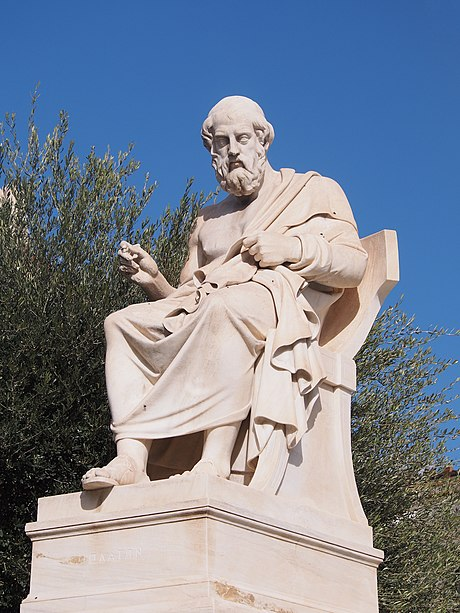
\includegraphics[width=4.5cm]{data/plato.JPG}
                };
            }
            \visible<2>{
                \node[inner sep=0pt, draw=black] at (0, 0) {
                    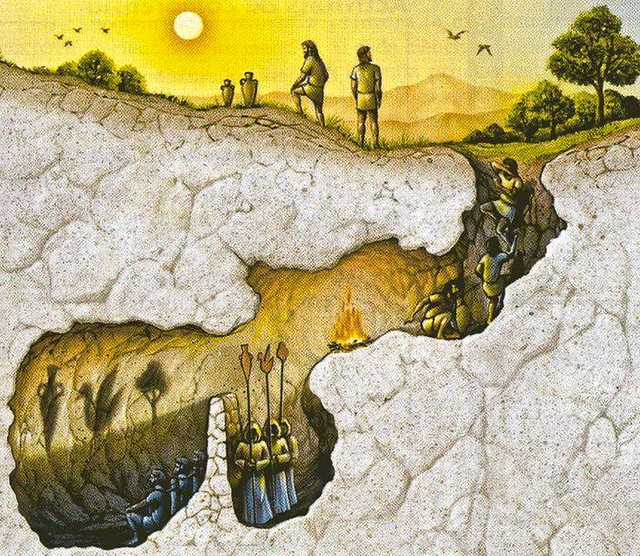
\includegraphics[width=7.5cm]{data/cave.jpg}
                };
            }
            \visible<3>{
                \node[inner sep=0pt, draw=black] at (0, 0) {
                    
\includegraphics[width=6cm]{data/kant.jpeg}
                };
            }
            \visible<4-5>{
                \node[inner sep=0pt, draw=black] at (-2.675, 0) {
                    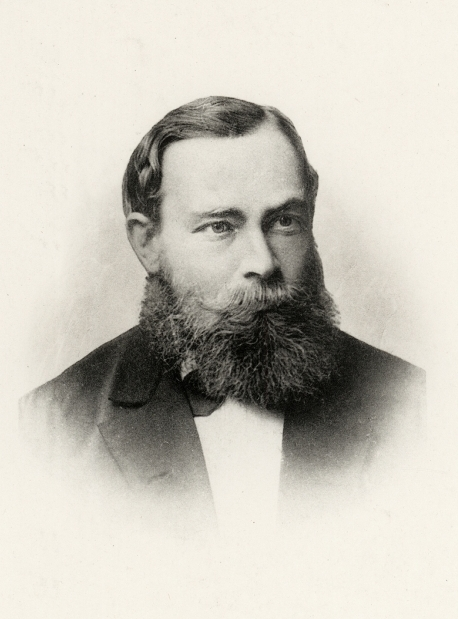
\includegraphics[height=5cm]{data/frege.jpg}
                };
            }
            \visible<5>{
                \node[inner sep=0pt, draw=black] at (2.675, 0) {
                    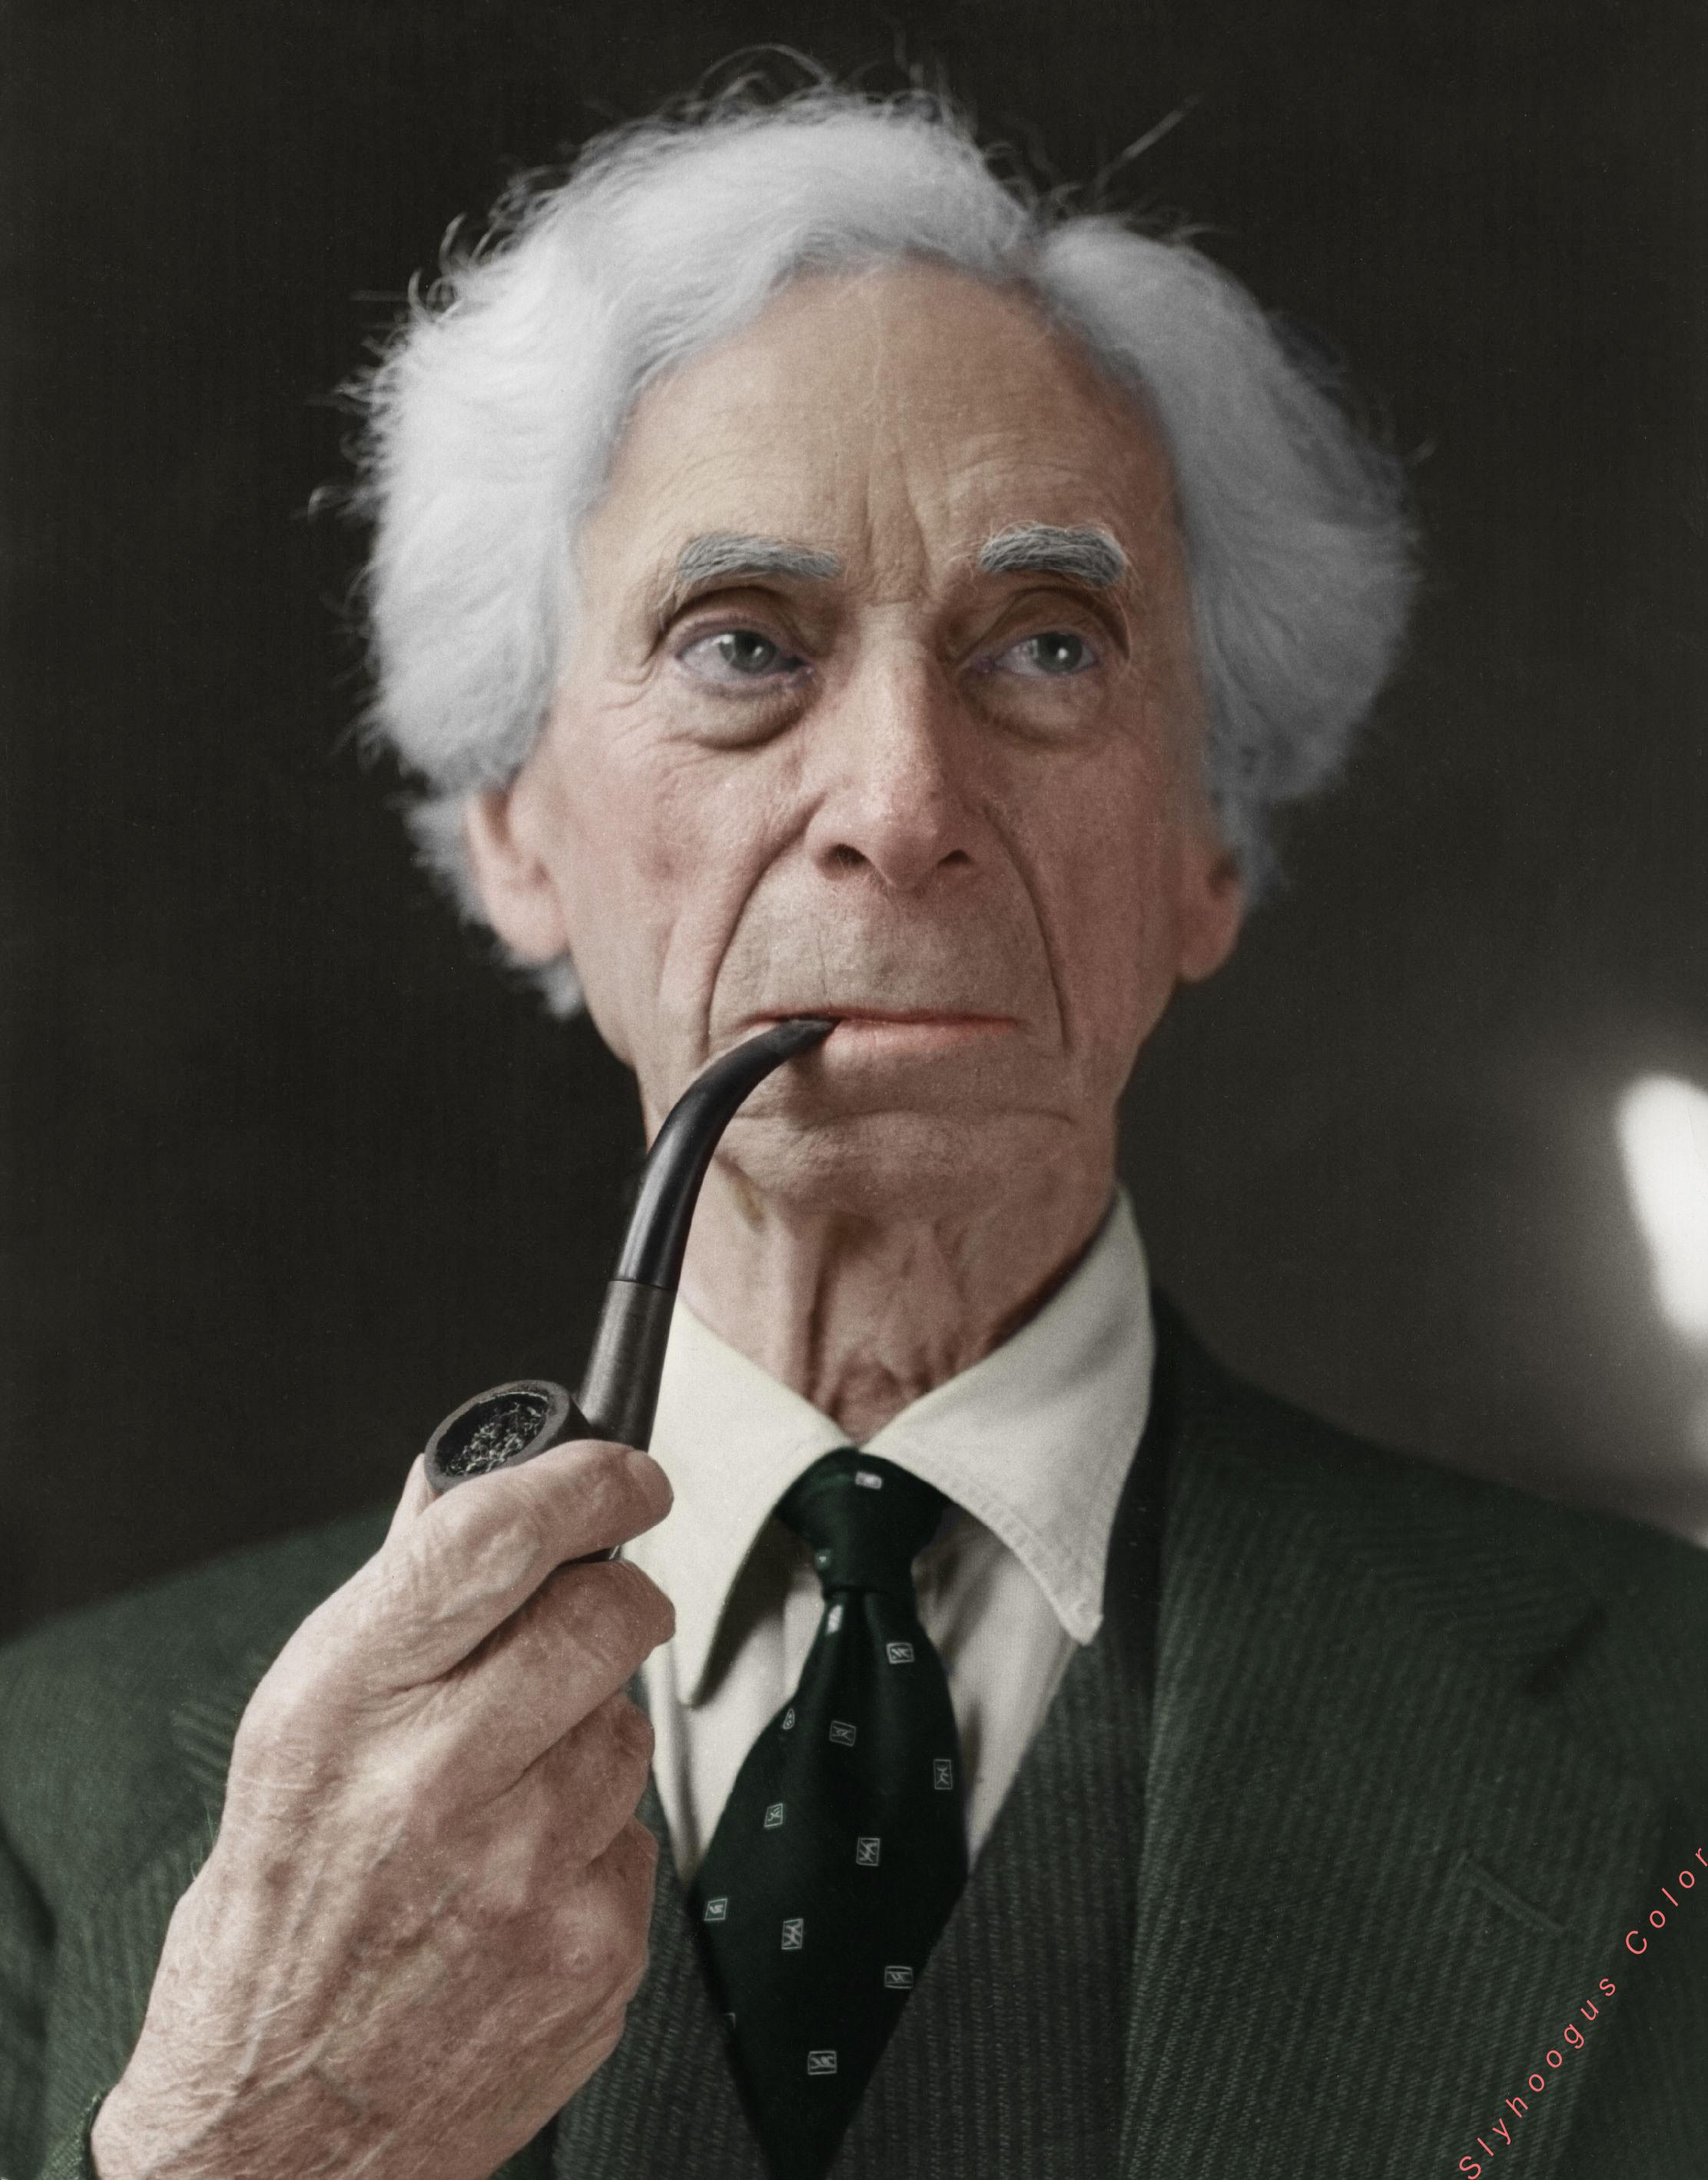
\includegraphics[height=5cm]{data/russell.jpg}
                };
            }
        \end{tikzpicture}
    \end{frame}

    \begin{frame}{The project}
        \begin{tikzpicture}
            \node[] at (-5.25, -3.5) {};
            \node[] at (5.25, 3.5) {};

            \visible<1-2>{
                \node[align=center] (functions) at (-2.675, -1) {
                    $x+y=z$\\$x-y=z$\\\ldots
                };
                \node[] (numbers) at (-2.675, 1) {
                    $0, 1, 2, 3, 4, \ldots$
                };
            }
            \visible<2>{
                \node[] at (0, 1) {
                    $\implies$
                };
                \node[] at (0, -1) {
                    $\implies$
                };
                \node[] at (2.675, 1) {
                    \large{\emoji{thinking-face}}
                };
                \node[] at (2.675, -1) {
                    \large{\emoji{check-mark-button}}
                };
            }
        \end{tikzpicture}
    \end{frame}

    \begin{frame}{Set theory}
        \begin{tikzpicture}
            \node[] at (-5.25, -3.5) {};
            \node[] at (5.25, 3.5) {};

            \visible<1>{
                \node[inner sep=0pt, draw=black] at (0, 0) {
                    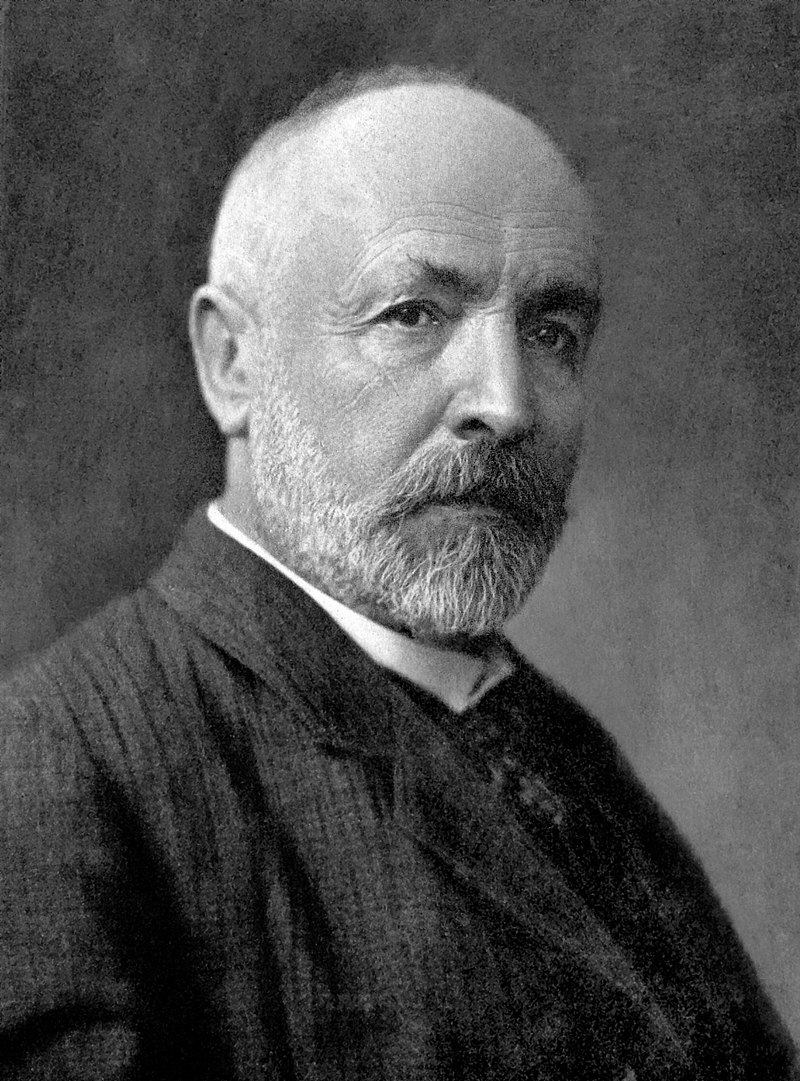
\includegraphics[width=5cm]{data/cantor.jpg}
                };
            }
            \visible<2>{
                \node[] at (0, 1.5) {
                    \{\emoji{nerd-face}, \emoji{woman}, \emoji{girl}, \emoji{dog-face}\}
                };
                \node[] at (0, 0.5) {
                    \{\emoji{nerd-face}, \emoji{smiling-face-with-sunglasses}, \emoji{face-with-monocle}, \emoji{woman-scientist},
                    \emoji{woman-technologist}, \emoji{woman-teacher}\}
                };
                \node[align=center] at (0, -0.5) {
                    \{monday, tuesday, wednesday, thursday,\\friday, saturday, sunday\}
                };
                \node[] at (0, -1.5) {
                    \{\emoji{laptop}, \emoji{mobile-phone}\}
                };
            }
            \visible<3>{
                \node[align=center] at (0, 0) {
                    \{\emoji{nerd-face}, \emoji{woman}, \emoji{girl}\}\\
                    \{\emoji{soccer-ball}, \emoji{basketball}, \emoji{volleyball}\}\\
                    \{tuesday, thursday, saturday\}\\
                    \ldots
                };
            }
            \visible<4>{
                \node[] at (0, 1) {
                    $\{1, 3, 5\}$
                };
                \node[] at (0, 0) {
                    $\{1, 10, 100\}$
                };
                \node[align=center] at (0, -1) {
                    $\{\}$
                };
            }
            \visible<5-6>{
                \node[] at (0, 0.5) {
                    $\{1, 2, 3, \ldots\}$
                };
            }
            \visible<6>{
                \node[] at (0, -0.5) {
                    $\{x\ |\ x > 0\}$
                };
            }
            \visible<7>{
                \node[] at (0, 0.5) {
                    $\{1, 3, 5, \ldots\}$
                };
                \node[] at (0, -0.5) {
                    $\{x\ |\ x\ \%\ 2\neq0\}$
                };
            }
            \visible<8-12>{
                \node[align=center] at (0, 1.5) {
                    \{\{\emoji{nerd-face}, \emoji{woman}, \emoji{girl}, \emoji{dog-face}\}, \{\emoji{nerd-face}, \emoji{smiling-face-with-sunglasses}, \emoji{face-with-monocle}, \emoji{woman-scientist},
                    \emoji{woman-technologist}, \emoji{woman-teacher}\},\\\{monday, tuesday, wednesday, thursday, friday, saturday, sunday\},\\\{\emoji{laptop}, \emoji{mobile-phone}\}, $\{1, 3, 5\}$, $\{1, 10, 100\}$, $\{\}$, $\{x\ |\ x > 0\}$, $\{x\ |\ x\ \%\ 2\neq0\}$\}
                };
            }
            \visible<9-12>{
                \node[] at (0, 0) {
                    $\{\{\}, \{0\}, \{1\}, \{0, 1\}, \ldots\}$
                };
            }
            \visible<10-12>{
                \node[] (s) at (0, -1) {
                    $\{x\ |\ x \mathrm{\ is\ a\ set}\}$
                };
            }
            \visible<11-12>{
                \node[anchor=east] at ($ (s.west) + (0.2, 0) $) {
                    $S=$
                };
            }
            \visible<12>{
                \node[] at (0, -2) {
                    $S \in S\ ?$
                };
            }
            \visible<13-16>{
                \node[] at (-2.5, 1) {
                    $S=\{\{\}, \{0\}, \{1\}, \{0, 1\}, \ldots, S, \ldots\}$
                };
                \node[] at (-2.5, 0) {
                    $S \in S$
                };
            }
            \visible<14-16>{
                \node[] at (2.5, 1) {
                    $S=\{1, 3, 5\}$
                };
                \node[] at (2.5, 0) {
                    $S \notin S$
                };
            }
            \visible<15-16>{
                \node[] at (0, -1.5) {
                    $\{S\ |\ S \in S\}$
                };
            }
            \visible<16>{
                \node[] at (0, -2) {
                    $\{S\ |\ S \notin S\}$
                };
            }

            \visible<17-22>{
                \node[] at (0, 1.5) {
                    $T=\{S\ |\ S \notin S\}$
                };
            }
            \visible<18-22>{
                \node[] (q) at (0, 0.5) {
                    $T \in T\ ?$
                };
            }
            \visible<19-22>{
                \node[] (no) at (-1.5, -1) {
                    No ($T \notin T$)
                };
                \draw[-stealth] (q) -- (no);
            }
            \visible<20-22>{
                \node[] (no2) at (-1.5, -2) {
                    Yes
                };
                \draw[-stealth] (no) -- (no2);
            }
            \visible<21-22>{
                \node[] (yes) at (1.5, -1) {
                    Yes ($T \in T$)
                };
                \draw[-stealth] (q) -- (yes);
            }
            \visible<22>{

                \node[] (yes2) at (1.5, -2) {
                    No
                };
                \draw[-stealth] (yes) -- (yes2);
            }
            \visible<23>{
                \node[inner sep=0pt, draw=black] at (0, 0) {
                    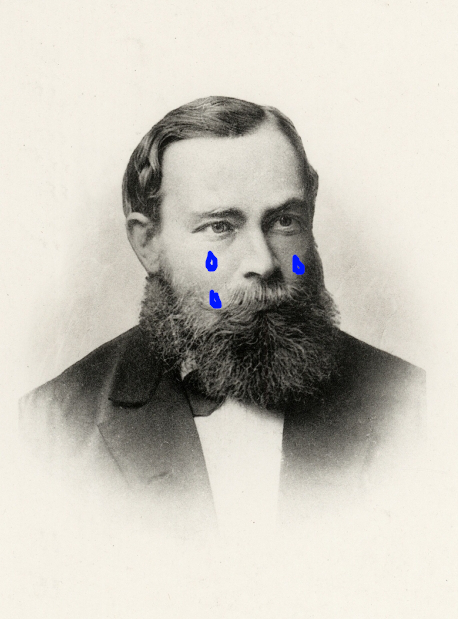
\includegraphics[height=6cm]{data/fregecry.jpg}
                };
            }
            \visible<24>{
                \node[align=center, text width=10cm, align=flush center] at (0, 0) {
                    \textit{"Hardly anything more unfortunate can befall a scientific writer than to have one of the foundations of his edifice shaken after the work is finished. This was the position I was placed in by a letter of Mr. Bertrand Russell, just when the printing of this volume was nearing its completion."}
                };
            }
        \end{tikzpicture}
    \end{frame}

    \begin{frame}{Gödels incompleteness theorem}
        \begin{tikzpicture}
            \node[] at (-5.25, -3.5) {};
            \node[] at (5.25, 3.5) {};

            \visible<1>{
                \node[inner sep=0pt, draw=black] at (0, 0) {
                    \includegraphics[width=5cm]{data/gødel.jpg}
                };
            }
            \visible<2-3>{
                \node[text width=5cm] at (-2.675, 1.5) {
                    \begin{enumerate}
                        \item 0 is a natural number
                        \item If $n$ is a natural number, $S(n)$ is a natural number
                        \item No numbers have 0 as their successor
                    \end{enumerate}
                };

                \node[text width=5cm, align=center] at (2.675, 1.5) {
                    $
                    \begin{aligned}
                        0&\\
                        1&=S(0)\\
                        2&=S(S(0))\\
                        &\ldots
                    \end{aligned}
                    $
                };
            }
            \visible<3>{
                \node[text width=5cm] at (-2.675, -1.5) {
                    \begin{enumerate}
                        \item[4] If $f(0)$ exists and $f(x+1)$ holds whenever $f(x)$ holds, $f$ is a valid function
                    \end{enumerate}
                };
                \node[text width=5cm, align=center] at (2.675, -1.5) {
                    $
                    \begin{aligned}
                        x+0&=x\\
                        x+S(y)&=S(x+y)
                    \end{aligned}
                    $
                };
            }
            \visible<4>{
                \node[text width=10cm, align=center] at (0, 0) {
                    $
                    \begin{aligned}
                        0 &:= 2\\
                        S(0) &:= 12965404\\
                        S(S(0)) &:= 24300749247875100
                    \end{aligned}
                    $
                };
                \node[text=red] at (1, -1.5) {
                    Gödel number
                };
                \draw[red, -stealth] (1, -1.3) -- (1, -0.8);
            }
            \visible<5-6>{
                \node[text width=10cm, align=center] at (0, 0) {
                    $x$ is not provable
                };
                \node[text=red] at (-1.35, 1) {
                    A valid gödel number
                };
                \draw[red, -stealth] (-1.35, 0.8) -- (-1.35, 0.3);
            }
            \visible<6>{
                \node[text=red] at (0, -1) {
                    $x$
                };
                \draw[red, -stealth] (0, -0.8) -- (0, -0.3);
            }
        \end{tikzpicture}
    \end{frame}

    \begin{frame}{The halting problem}
        \begin{tikzpicture}
            \node[] at (-5.25, -3.5) {};
            \node[] at (5.25, 3.5) {};

            \visible<1>{
                \node[inner sep=0pt, draw=black] at (0, 0) {
                    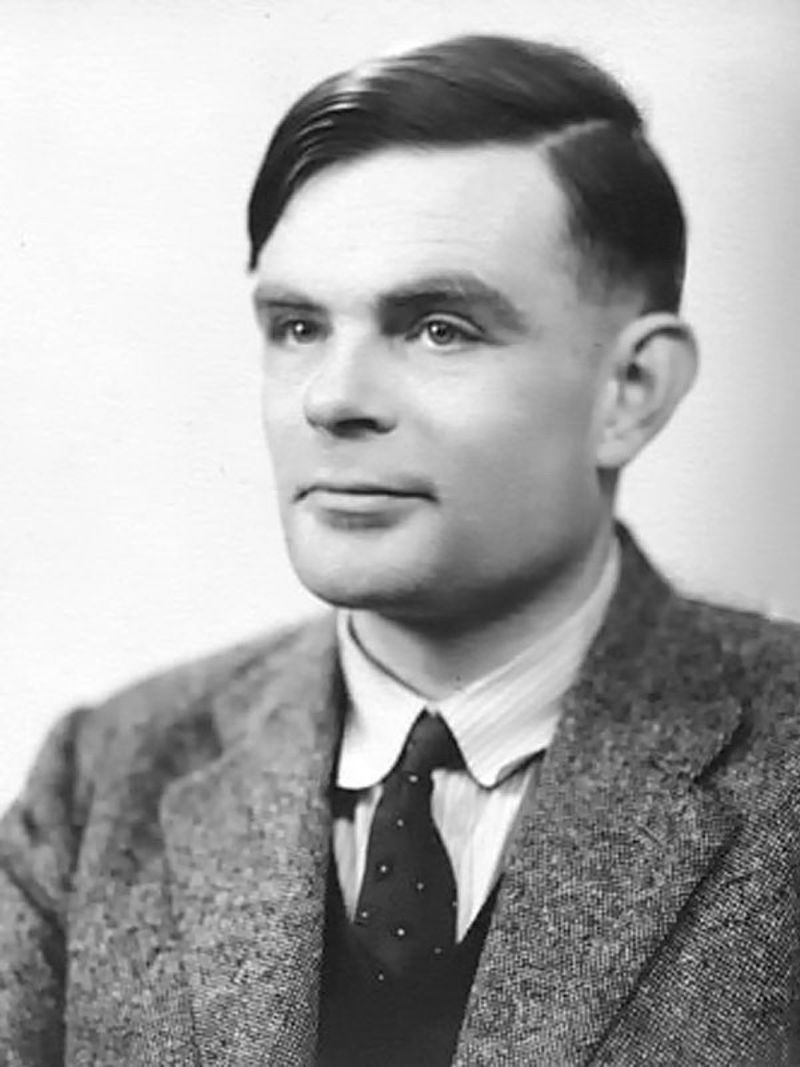
\includegraphics[width=5cm]{data/turing.jpg}
                };
            }
            \visible<2-3>{
                \node[text width=10cm, align=flush left] at (0, 1) {
                    \textbf{The halting problem}\\
                    Given a program $P$ and an input $i$, determine if $P$ halts on $i$
                };
            }
            \visible<3>{
                \node[] (halt) at (-2.675, -1) {
                    print('Hello world')
                };
                \node[align=left] (nohalt) at (2.675, -1) {
                    while True:\\
                    \ \ \ \ print('Hello world')
                };
                \node[text=green] (yes) at (-2.675, -2.5) {
                    Halts
                };
                \node[text=red] (no)at (2.675, -2.5) {
                    Does not halt
                };
                \draw[green, -stealth] (halt) -- (yes);
                \draw[red, -stealth] (nohalt) -- (no);
            }
            \visible<4>{
                \PythonInputNode{1}{(-4, 3)}{pythonnode}{0.9\textwidth}{7}{
                    def decider(program, input):^^J
                    { }{ }{ }{ }"""Magical function that decides whether the program^^J
                    { }{ }{ }{ }halts on the input"""^^J
                    { }{ }{ }{ }...^^J
                }
            }
            \visible<5-6>{
                \PythonInputNode{1}{(-4, 3)}{pythonnode}{0.9\textwidth}{7}{
                    def decider(program, input):^^J
                    { }{ }{ }{ }"""Magical function that decides whether the program^^J
                    { }{ }{ }{ }halts on the input"""^^J
                    { }{ }{ }{ }...^^J
                    ^^J
                    def f(program):^^J
                    { }{ }{ }{ }if decider(program, program):^^J
                    { }{ }{ }{ }{ }{ }{ }while True: pass^^J
                    { }{ }{ }{ }else:^^J
                    { }{ }{ }{ }{ }{ }{ }return^^J
                    ^^J
                    f(f)
                }
            }
            \visible<6>{
                \node[thick, draw=red, minimum height=0.3cm, minimum width=0.6cm, inner sep=0pt] at (-3.52, -0.35) {};
            }
        \end{tikzpicture}
    \end{frame}

    \begin{frame}{Summary}
        \textbf{There are limits to what we can do with formal approaches}\\
        \begin{itemize}
            \item These typically break down in the presence of self-references
        \end{itemize}
    \end{frame}

    \begin{frame}{Are we all strange loops?}
        \begin{tikzpicture}
            \node[] at (-5.25, -3.5) {};
            \node[] at (5.25, 3.5) {};

            \visible<1>{
                \node[inner sep=0pt, draw=black] at (0, 0) {
                    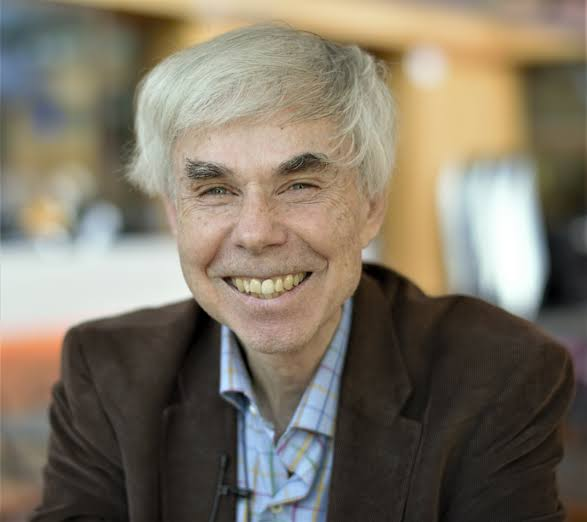
\includegraphics[width=6cm]{data/hofstadter.jpeg}
                };
            }
            \visible<2>{
                \node[inner sep=0pt, draw=black] at (0, 0) {
                    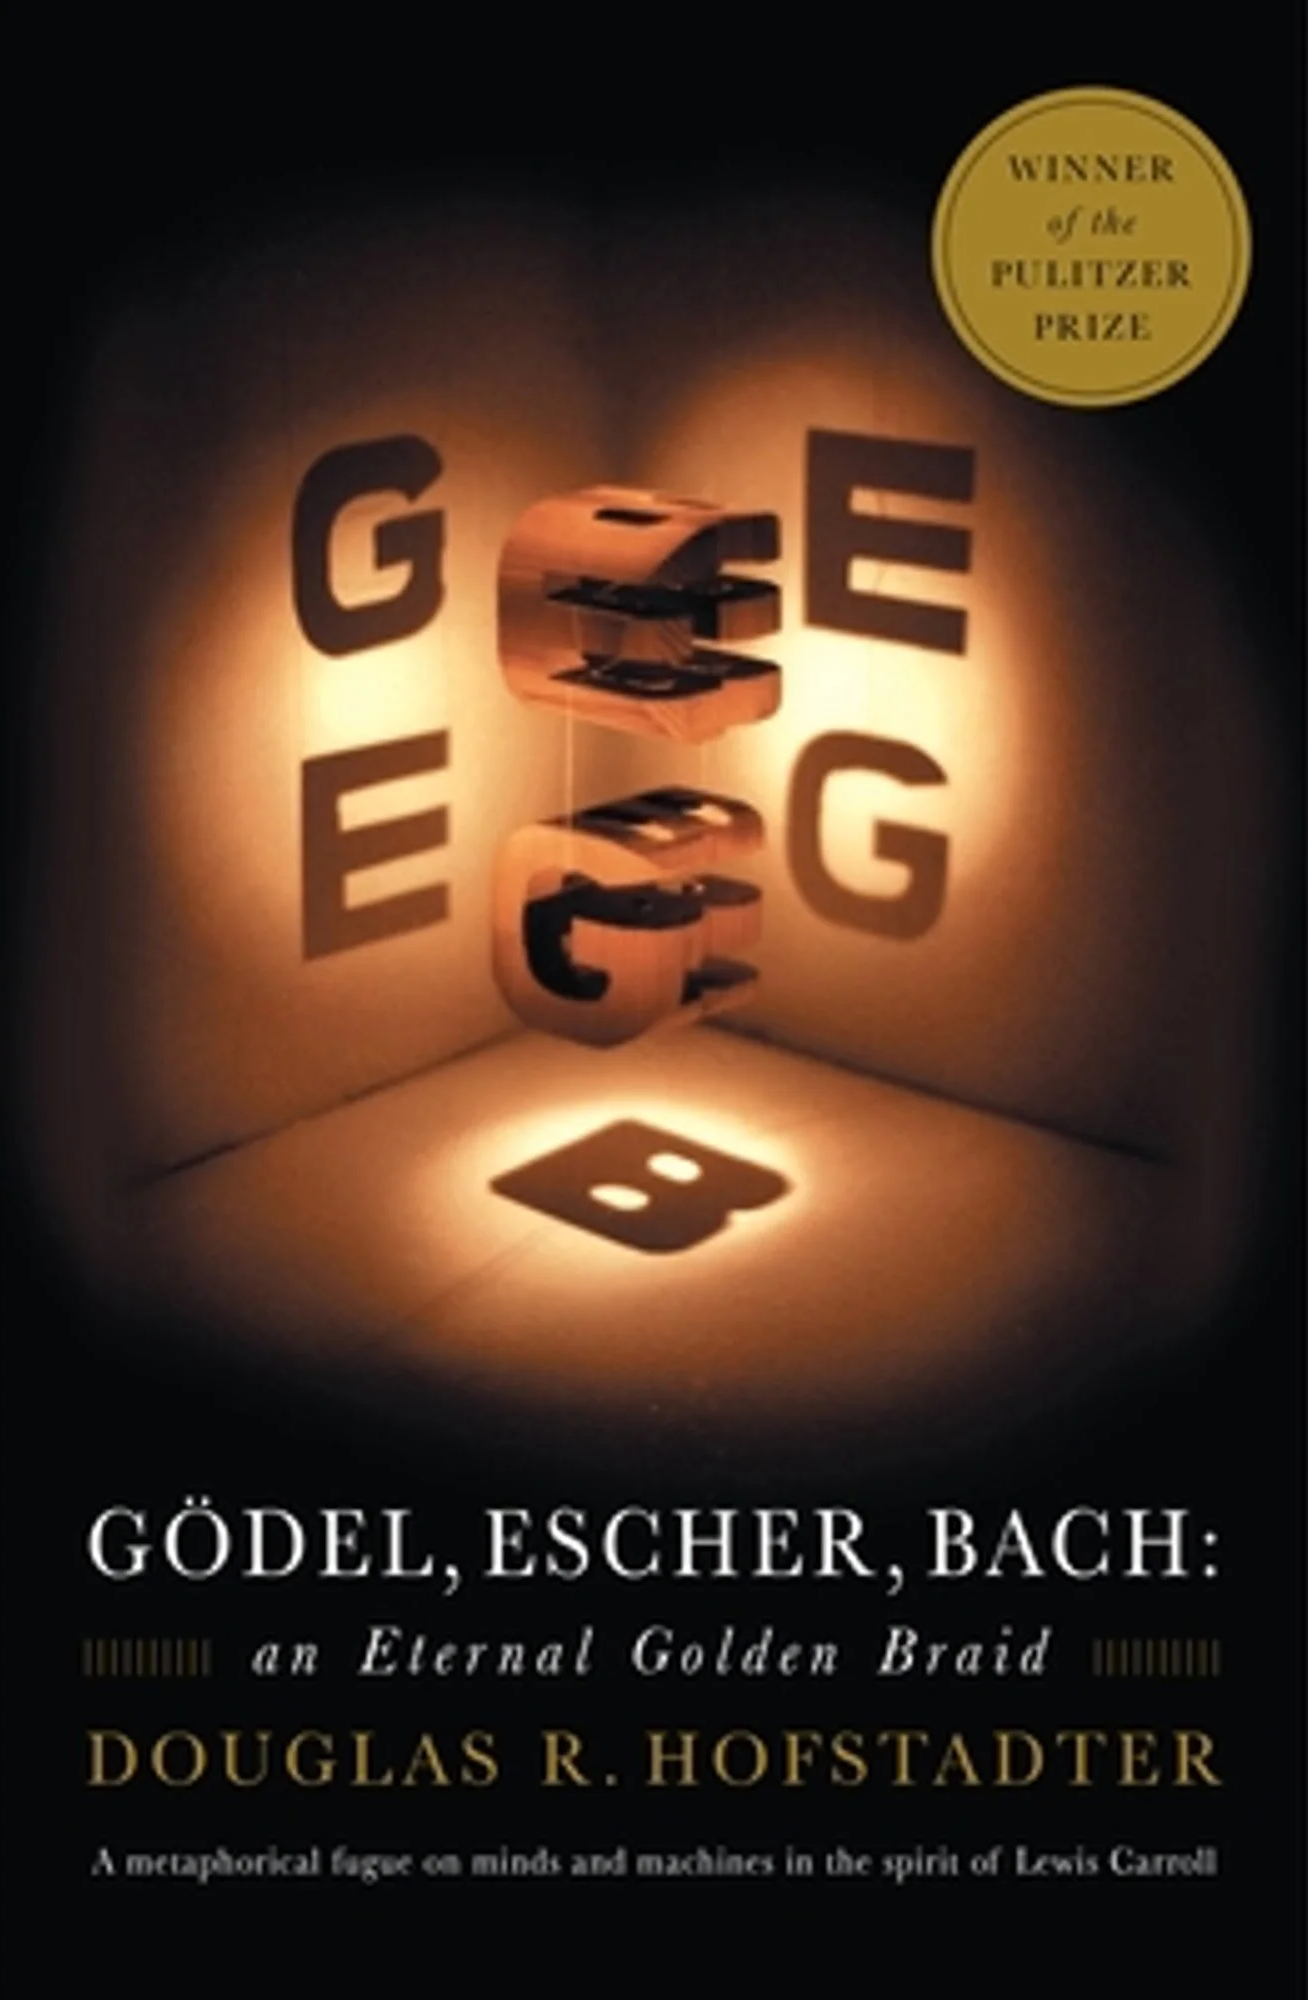
\includegraphics[width=4cm]{data/geb.png}
                };
            }
            \visible<3>{
                \node[inner sep=0pt, draw=black] at (0, 0) {
                    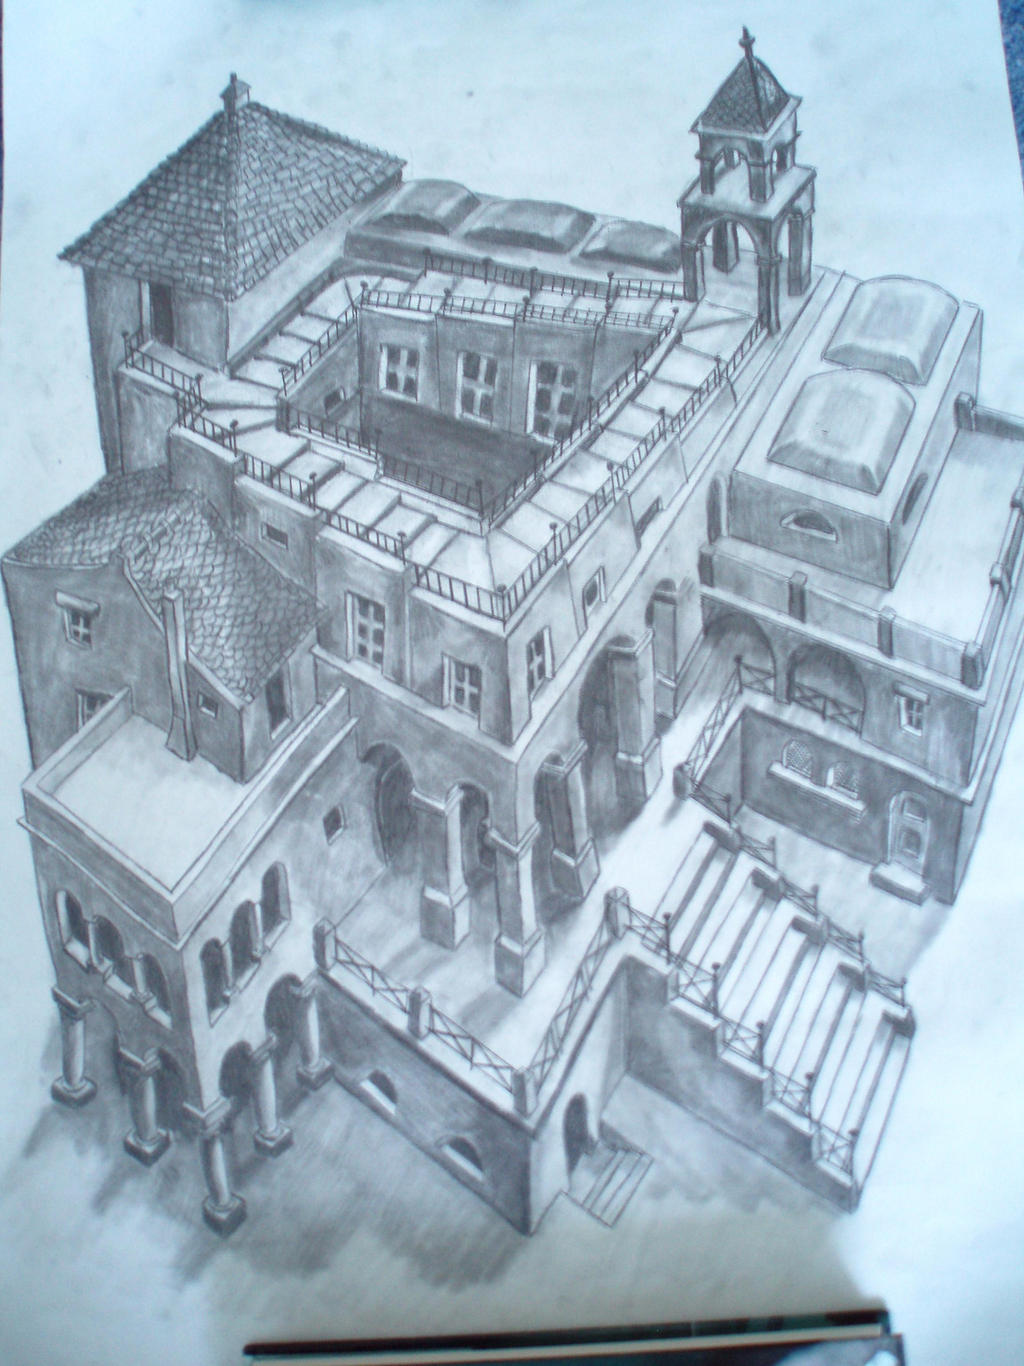
\includegraphics[width=5cm]{data/stairs.jpg}
                };
            }
            \visible<4>{
                \node[inner sep=0pt, draw=black] at (0, 0) {
                    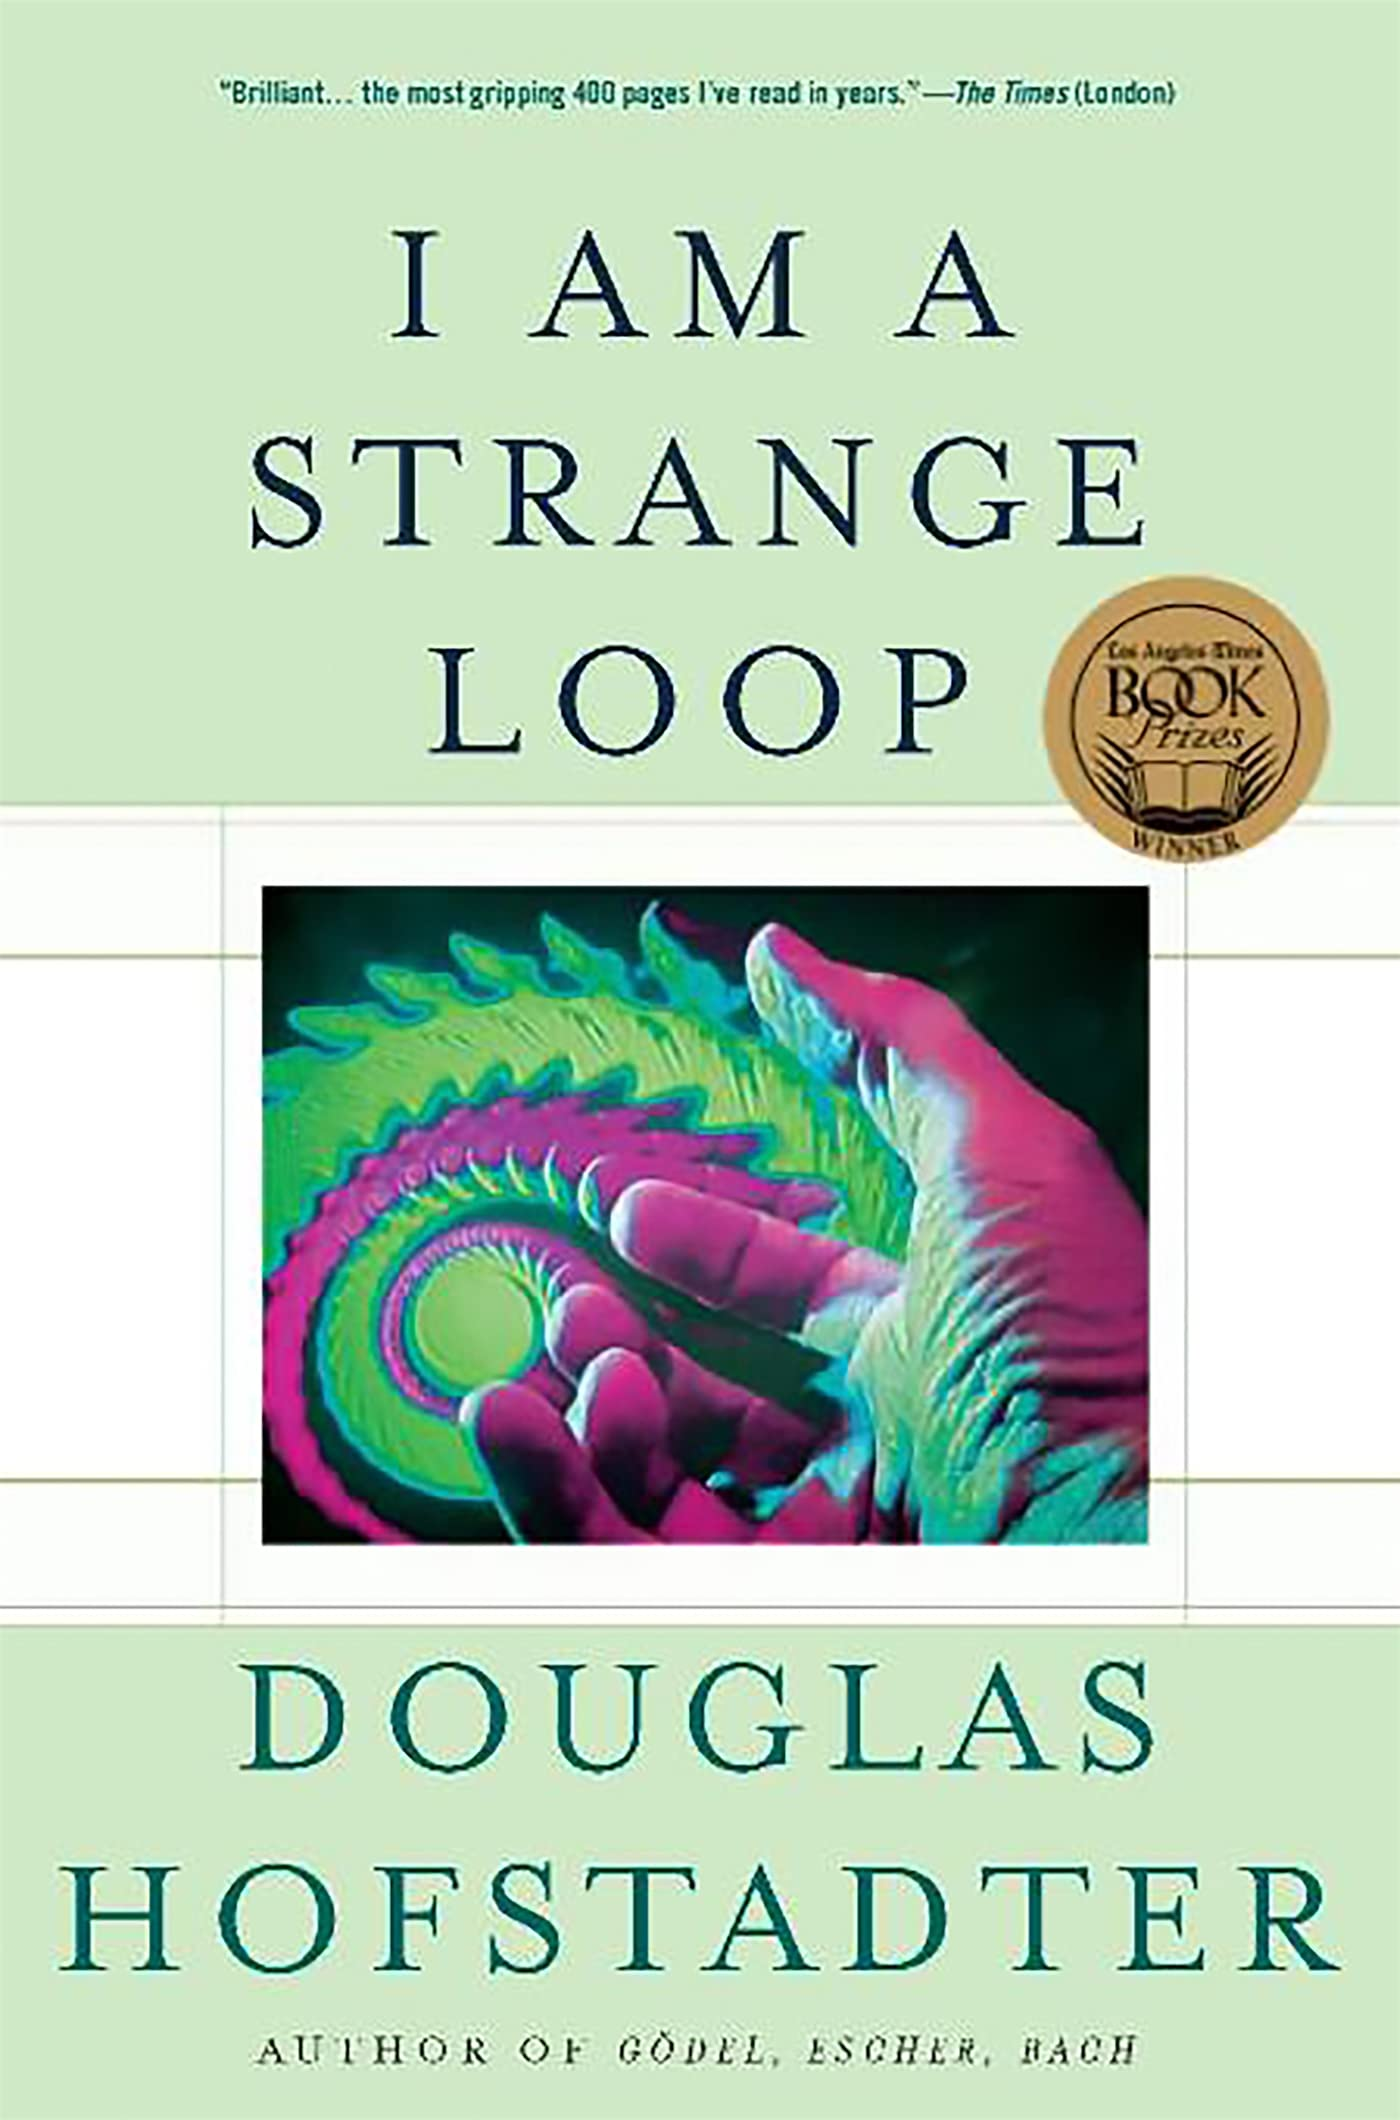
\includegraphics[width=4.5cm]{data/loop.jpg}
                };
            }
            \visible<5>{
                \node[inner sep=0pt, draw=black] at (0, 0) {
                    
\includegraphics[width=4cm]{data/humanbrain.png}
                };
            }
            \visible<6>{
                \node[inner sep=0pt, draw=black] at (0, 0) {
                    
\includegraphics[width=4cm]{data/DoloresAbernathy.png}
                };
            }
        \end{tikzpicture}
    \end{frame}

\end{document}
